\documentclass[11pt, a4paper]{article}

% Packages
\usepackage[french]{babel}
\usepackage[T1]{fontenc}
\usepackage[utf8]{inputenc}

\usepackage[left=2cm, right=2cm, top=2cm, bottom=2cm]{geometry}
\usepackage{fancyhdr}
\usepackage{lastpage}
\usepackage{hyperref}

\usepackage{float}

\usepackage{graphicx}
\graphicspath{{./img/}}
\usepackage{tikz}

% Reset paragraph indentation -------------------------------------------------
\setlength{\parindent}{0cm}

% Allow a paragraph to have a linebreak ---------------------------------------
\newcommand{\paragraphnl}[1]{\paragraph{#1}\mbox{}\\}

% Page header and footer ------------------------------------------------------
\pagestyle{fancy}
\setlength{\headheight}{33pt}
\renewcommand{\headrulewidth}{0.5pt}
\lhead{
\includegraphics[height=1cm]{hepia.jpg}}
\chead{SmartFolder}
\rhead{Claudio Sousa - David Gonzalez}
\renewcommand{\footrulewidth}{0.5pt}
\lfoot{26 janvier 2017}
\cfoot{}
\rfoot{Page \thepage /\pageref{LastPage}}

% Table of contents depth -----------------------------------------------------
\setcounter{tocdepth}{3}

% Document --------------------------------------------------------------------
\begin{document}

\title
{
    \Huge{Programmation système} \\
    \Huge{SmartFolder}
}
\author
{
    \LARGE{David Gonzalez - Claudio Sousa}
}
\date{26 janvier 2017}
\maketitle

\begin{center}
    %\includegraphics[scale=0.27]{logo.png}
\end{center}

\thispagestyle{empty}

\newpage

% -----------------------------------------------------------------------------
\section{Introduction}

Ce TP de deuxième année en programmation système consiste à implémenter un programme similaire au SmartFolder sur MacOSX. \\

Le SmartFolder sur MacOSX recherche sur le disque des fichiers correspondant à un/des critères et,
pour chacun des fichiers trouvés, le programme crée un lien symbolique dans un dossier specifié.

\subsection{Spécification fonctionnelle}
Ce programme possède deux modes de fonctionnement.

\subsubsection{Mode recherche}
C'est le mode par défaut et simule le SmartFolder sur MacOSX. \\

Dans ce mode, le programme tourne en arrière-plan et maintient dans le dossier de destination une liste de liens vers les fichier trouvés correspondant aux critères de recherche choisis.
Cette liste est dynamique et mise à jour si des nouveaux fichiers répondent aux critères de recherche ou si, au contraire, des fichiers ne répondent plus à ces critères. \\

La recherche de fichiers est récursive et suit les liens symboliques.

Par ailleurs, les fichiers en double ne doivent pas apparaître et les fichiers portant le même nom doivent être renommés intelligemment. \\

Ce mode prend 3 paramètres:
\begin{itemize}
    \item \textit{<dir\_name>}: chemin (de destination) où stocker les liens;
    \item \textit{<search\_path>}: chemin de recherche;
    \item \textit{<expression>}: critères de sélection. \\
\end{itemize}

\textit{<dir\_name>} et \textit{<search\_path>} sont de simples chemins vers des dossiers.\\
\textit{<expression>} correspond à une liste de critères dont l'interface est un sous-ensemble de celle de \textit{find}. Son usage complet est décrit en annexe, section \nameref{ann_exp}.


\subsubsection{Mode stop}
Le mode \textit{stop} permet d'arrêter une recherche en cours. \\

Ce mode prend en paramètre:
\begin{itemize}
	\renewcommand\labelitemi{}
    \item \textit{-d} \textit{<dir\_name>}: termine le SmatFolder pour le chemin de destination specifié.
\end{itemize}

\newpage

% -----------------------------------------------------------------------------
\section{Development}
\subsection{Architecture}

\begin{figure}[H]
    \begin{center}
        \includegraphics[width=\textwidth]{modules.png}
    \end{center}
    \caption{Architecture du SmartFolder}
    \label{Architecture du SmartFolder}
\end{figure}

\newpage

\subsubsection{Main}

Le programme principal a pour rôle de vérifier les arguments et de sélectionner le bon mode de fonctionnement.

Dans le mode \textit{recherche}, il a pour tâche de:
\begin{itemize}
    \item met le processus en arrière-plan;
    \item demande au module \textit{Parser} de traiter l'expression;
    \item initialise le module \textit{IPC};
    \item initialise et lance le module \textit{SmartFolder}.\\
\end{itemize}

Dans le mode \textit{stop}, son seul rôle est de signaler l'arrêt à l'autre instance (voir \nameref{sec:ipc}).

\subsubsection{SmartFolder}
\textit{SmartFolder} est le module principal qui va orchestrer la recherche et la mise à jour du dossier de destination. \\

Lorsque lancé, il va continuellement utiliser le module \textit{Finder} pour rechercher les fichiers correspondant au critère,
puis donner la liste des fichiers retournée au module \textit{Linker} pour qu'il mette à jour le répertoire de destination.

A noter qu'entre chaque recherche, il y a une pause de quelques secondes. \\

A l'arrêt, il est chargé de détruire le répertoire de destination et de libérer ses ressources.

\subsubsection{Parser}
\textit{Parser} est le module qui transforme
l'expression spécifiée dans la ligne de commande (critères de recherche) en une structure interne utilisable par le module \textit{Validator}. \\

La complexité des différents opérateurs logiques possibles (priorité, parenthèses, opérateur unaire) doit être connue uniquement de ce module. La structure retournée doit pouvoir être traitée simplement par le module \textit{Validator}. \\

Suggestion d'implémentation: utiliser l'algorithme de \textit{shunting-yard}\footnote{\url{https://en.wikipedia.org/wiki/Shunting-yard\_algorithm} (par Edsger Dijkstra)} pour le traitement de l'expression.

\subsubsection{Validator}
Ce module vérifie si un fichier est valide selon l'expression créée par le module \textit{Parser}.

\subsubsection{Finder}
Ce module est responsable de produire la liste de tous les fichiers du dossier de recherche respectant les criteres de recherche.

La vérification des fichiers contre les critères est déleguée au module \textit{Validator}.\\

Lors du processus de recherche effectué au sein de ce module, un parcours d'arborescence est effectué récursivement et les liens symboliques sont suivis.

Des boucles deviennent alors possibles. Ce module doit donc gérer ce cas spécifique et prévenir les boucles infinies ainsi que le traitement des fichiers et dossiers dupliqués. \\

Possibilité d'implémentation: utilisation d'une table d'hashage contenant les numéros d'inode des fichiers et répertoires déjà parcourus.

\subsubsection{Linker}
Le module \textit{Linker} a pour rôle de mettre à jour le dossier de destination
à l'aide d'une liste de fichiers passée en paramètre. \\

Pour chaque fichier, il crée un lien si celui-ci n'existe pas. Les liens qui ne sont plus valides sont effacés.

\subsubsection{IPC}
\label{sec:ipc}
Ce module a pour but de répondre au problème du mode \textit{stop}.
En effet, lorsqu'une instance de \textit{SmartFolder} souhaite arrêter une autre instance en cours d'exécution,
il faut d'une manière ou d'une autre permettre une communication simple entre les deux processus afin
qu'une instance puisse signaler un arrêt à une autre instance. \\

Le moyen de communication choisi est les signaux POSIX, le signal \textit{SIGTERM} pour être plus précis.
Une instance qui veut donc signaler l'arrêt doit envoyer le signal cité au processus concerné. \\

Afin de pouvoir lancer un signal, il faut que le PID du processus cible soit connu.
Pour cela, le PID d'une instance en mode \textit{recherche} est stocké dans un fichier
dans le répertoire utilisateur.

Comme une instance de \textit{SmartFolder} est unique par dossier de destination,
ce fichier se nommera d'après le chemin de ce répertoire.

\subsubsection{IO}
Le but de ce module est d'offrir une interface simple aux appels systèmes et de centraliser la gestion des erreurs.

\subsubsection{Logger}
Ce module centralise l'affichage des logs de débogage.

\newpage

% -----------------------------------------------------------------------------
\subsection{Flux général d'exécution}

Le diagramme ci-dessous décrit le flux général de l'application:

\begin{figure}[H]
    \begin{center}
        \includegraphics[width=0.8\textwidth]{flow.png}
    \end{center}
    \caption{Flow général d'exécution}
    \label{Flow général d'exécution}
\end{figure}

L'application commence par décoder le premier argument pour savoir dans quel mode il doit être exécuté. \\

En mode \textit{recherche}, il commence par se mettre en arrière-plan.
Puis, il donne le reste des argument au Parser d'expression pour la validation des fichiers.
Ensuite, il écrit son PID dans le fichier et crée le dossier de destination donnée en argument pour pouvoir commencer la recherche. \\

La recherche tourne indéfiniment tant qu'un signal d'arrêt (SIGTERM ou SIGINT) n'est pas reçu.
Cette recherche commence par parcourir récursivement l'ensemble des fichiers dans le dossier de recherche donnée en argument.
Puis, avec cette liste, le programme met à jour les liens dans le dossier de destination en commençant par purger
les liens qui ne figurent plus dans la liste, puis crée ceux qui y sont nouveaux.
La recherche se termine par une attente de quelques secondes et recommence. \\

En mode \textit{stop}, il se contente de lire le PID dans le fichier créé par l'instance cible et
lui envoie un signal de terminaison (SIGTERM).
Ceci provoque l'exécution d'un \textit{handler} sur l'instance concernée qui place un indicateur
pour que la boucle de recherche s'arrête.

\newpage

% -----------------------------------------------------------------------------
\section{Implémentation}

La documentation d'implémentation a été générée à l'aide de \href{http://www.doxygen.org/index.html}{Doxygen} en version HTML et se trouve à l'addresse:
\url{https://hepia-projects.gitlab.io/smart-folder/}. \\

Tous les modules possèdent une description complète en début de fichier.
Toutes les fonctions publiques ont été documentées dans le fichier d'header,
alors que les fonctions privées ont été documentées dans le fichier d'implémentation. \\

Le diagramme d'architecture (figure \ref{Architecture du SmartFolder}) donne toutes les fonctions et structures publiques de chaque module. \\

Le code source, testes unitaires et source du rapport se trouve à l'adresse \url{https://gitlab.com/hepia-projects/smart-folder/tree/master}. \\

\subsection{Testes unitaires}

Le module \textit{Parser} a été entièrement testé à l'aide de \href{http://cutest.sourceforge.net/}{CuTest}.
Ce module fut choisit en raison de sa complexité.
Les tests unitaires se trouve dans le dossier \textit{tests} et peut être exécuté avec \textit{make run}. \\

L'image ci-dessous donne la sortie des tests unitaires du module \textit{Parser}:

\begin{figure}[H]
    \begin{center}
        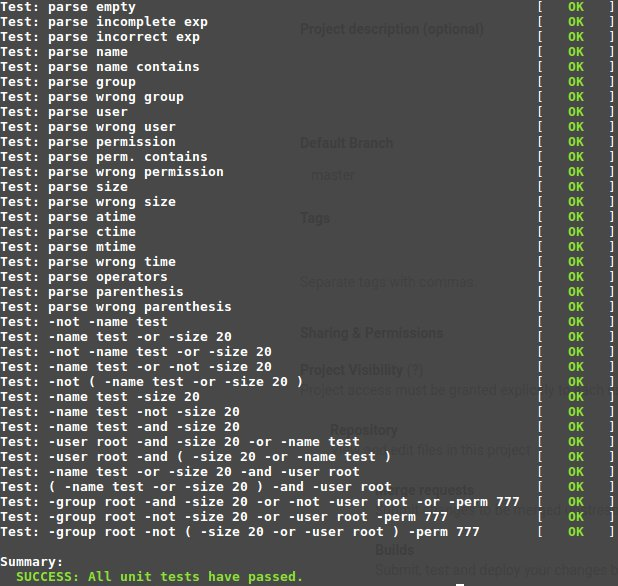
\includegraphics[width=0.8\textwidth]{unit_test_result.jpg}
    \end{center}
    \caption{Sortie des tests unitaires du module \textit{Parser}}
    \label{Sortie des tests unitaires du module Parser}
\end{figure}

\newpage

% -----------------------------------------------------------------------------
\section{Annexe}
\subsection{Expression}
\label{ann_exp}
L'interface est semblable à celle de \textit{find}\footnote{\url{https://linux.die.net/man/1/find}}.
Voici la liste des options prises en charge:\\

Critères:
\begin{itemize}
	\renewcommand\labelitemi{}
	\renewcommand\labelitemii{}
	\renewcommand\labelitemiii{}
	\item \textit{-name}: \underline{fname}
	\begin{itemize}
		\item Le nom de fichier est exactement \underline{fname}
		\item Exemple, les fichiers només  "todo.txt": \textit{-name todo.txt}
	\end{itemize}
	\item \textit{-name}: -\underline{fname}
	\begin{itemize}
		\item     Le nom de fichier contient \underline{fname}.
		\item     Exemple, les fichiers contenant ".txt":
		\textit{-name -.txt}
	\end{itemize}
	\item \textit{-group}: \underline{gname}
	\begin{itemize}
		\item 	   	Le fichier appartient au group \underline{gname}
		\item 	   	Exemple, les fichiers appartenant au group \textit{root}: \textit{-group root}
	\end{itemize}
	\item \textit{-user}: \underline{uname}
	\begin{itemize}
		\item 		Le fichier est possédé par utilisateur \underline{uname}
		\item 	   	Exemple, les fichiers possédés par l'utilisateur \textit{claudio}: \textit{-user claudio}
	\end{itemize}
	\item \textit{-perm}: \underline{perm}
	\begin{itemize}
		\item 		Les permissions sont exactement \underline{perm}
		\item 		Exemple, les fichiers ayant exactement les permissions 644: \textit{-perm 644}
	\end{itemize}
	\item \textit{-perm}: -\underline{perm}
	\begin{itemize}
		\item 		Le fichier a au moins les permissions \underline{perm}
		\item 		Exemple, les fichiers dont l'utilisateur peut lire et executer: \textit{-perm -500}
	\end{itemize}
	\item \textit{-size}: \underline{[+-]size[GMkc]}
	\begin{itemize}
		\item 		Le fichier a la taille \underline{size}.
		\item 		Le suffix indique l'unité utilisée (insensible à la casse):
		\begin{itemize}
			\item \textit{'c'}: bytes (par défaut si non précisé)
			\item \textit{'k'}: Kilobytes
			\item \textit{'M'}: Megabytes
			\item \textit{'G'}: Gigabytes
		\end{itemize}
		Le préfixe indique la comparaison utilisée:
		\begin{itemize}
			\item \textit{'+'}: supérieur à
			\item \textit{'-'}: inférieur à
			\item \textit{''}: exactement
		\end{itemize}
		Exemples:
		\begin{itemize}
			\item \textit{-size 200c}: fichiers de taille 200 bytes
			\item \textit{-size -30k}: fichiers de taille inférieure à 30KB
			\item \textit{-size +2M}: fichiers de taille supérieure à 2MB
		\end{itemize}
	\end{itemize}
	\item \textit{-atime}: \underline{[+-]time[dmhs]}
	\begin{itemize}
		\item	Le fichier fut accédé depuis \underline{time}. La référence de temps est le moment présent.
		\item	Le suffix indique l'unité utilisée (insensible à la casse):
		\begin{itemize}
            \item \textit{'s'}: secondes (par défaut si non précisé)
			\item \textit{'m'}: minutes
            \item \textit{'h'}: heures
			\item \textit{'d'}: jours
		\end{itemize}
		Le préfixe \textit{[+-]} indique la comparaison utilisée, comme pour le critère \underline{-size} ci-dessus.\\
		Exemples:
		\begin{itemize}
			\item \textit{-atime +5m}: fichiers accédés depuis plus de 5 minutes
			\item \textit{-atime -1d}: fichiers accédés dans les dernières 24 heures
		\end{itemize}
	\end{itemize}
	\item \textit{-ctime}: \underline{[+-]time[md]}
	\begin{itemize}
		\item 	Le statut du fichier fut changé depuis \underline{time}.
		\item Pour plus détails, voir l'explication pour le critère \underline{-atime}
	\end{itemize}
	\item \textit{-mtime}: \underline{[+-]time[md]}
	\begin{itemize}
		\item 	Le fichier fut changé depuis \underline{time}.\\
		Pour plus détails, voir l'explication pour le critère \underline{-atime} \\
	\end{itemize}
\end{itemize}

Les differents critères énumérés ci-dessus peuvent être combinés avec les opérateurs listés ci-dessous,
énumérés dans l'ordre de précédence décroissante: \\

Opérateurs:
\begin{itemize}
	\renewcommand\labelitemi{}
	\item \textit{( critère )}: force la précédence de l'expression entre parenthèses
	\item \textit{-not}: applique le \textit{NOT} logique  au critère de droite
	\item \textit{-and}: applique le \textit{AND} logique entre les critères à gauche et à droite de l'opérateur
	\item \textit{-or}: applique le \textit{OR} logique  entre les critères à gauche et à droite de l'opérateur
\end{itemize}

\newpage

% -----------------------------------------------------------------------------
\subsection{Changelog}

La liste ci-dessous décrit l'ensemble des changements apportés à ce document d'architecture.

\begin{itemize}
    \item mise à jour du diagramme pour l'ajout de:
    \begin{itemize}
        \item IO:
        \begin{itemize}
            \item structure: \textit{io\_file\_list};
            \item fonction: \textit{io\_file\_write\_fd};
            \item fonction: \textit{io\_directory\_get\_all};
            \item fonction: \textit{io\_directory\_create\_parent};
            \item fonction: \textit{io\_directory\_delete};
            \item fonction: \textit{io\_link\_exists}.
        \end{itemize}
    \end{itemize}
    \begin{itemize}
        \item Logger:
        \begin{itemize}
            \item fonction: \textit{logger\_debug};
            \item fonction: \textit{logger\_info};
            \item fonction: \textit{logger\_error};
            \item fonction: \textit{logger\_perror}.
        \end{itemize}
    \end{itemize}
    \begin{itemize}
        \item Parser:
        \begin{itemize}
            \item énumération: \textit{parser\_crit\_type\_t};
            \item énumération: \textit{parser\_crit\_t};
            \item énumération: \textit{parser\_comp\_t};
            \item fonction: \textit{parser\_free}.
        \end{itemize}
    \end{itemize}
    \begin{itemize}
        \item SmartFolder: renommé en SearchFolder.
    \end{itemize}
    \item ajout d'une section \textit{Flux général d'exécution};
    \item ajout d'une section \textit{Implémentation};
    \item Expression:
    \begin{itemize}
        \item les suffixes de taille (\textit{size}) sont insensibles à la casse.
        \item si le suffixe de taille (\textit{size}) n'est pas précisé, alors l'unité par défaut est l'octet (byte).
        \item ajout de deux suffixe de temps (\textit{atime}, \textit{ctime}, \textit{mtime}): 's' pour seconde et 'h' pour heures.
        \item les suffixes de temps (\textit{atime}, \textit{ctime}, \textit{mtime}) sont insensibles à la casse.
        \item si le suffixe de temps (\textit{atime}, \textit{ctime}, \textit{mtime}) n'est pas précisé, alors l'unité par défaut est la seconde.
    \end{itemize}
\end{itemize}

\end{document}
